\documentclass[final]{article}


\usepackage{APS360}
\usepackage[utf8]{inputenc} % allow utf-8 input
\usepackage[T1]{fontenc}    % use 8-bit T1 fonts
\usepackage{hyperref}       % hyperlinks
\usepackage{url}            % simple URL typesetting
\usepackage{booktabs}       % professional-quality tables
\usepackage{amsfonts}       % blackboard math symbols
\usepackage{nicefrac}       % compact symbols for 1/2, etc.
\usepackage{microtype}      % microtypography
\usepackage{xcolor}         % colors
\usepackage{graphicx}
 
\title{Clash of Clans Base Archetype Classifier}

\author{%
  Saptarshi Talukdar \\
  1010662757, saptarshi.talukdar@mail.utoronto.ca\\
  \textbf{Colab Notebook:} \url{https://tinyurl.com/4928ku8s}\\
  \textbf{GitHub Link:} \url{https://github.com/SattiDaBeaver/APS360-Project}\\
}

\begin{document}

\maketitle

\vspace{-0.5in}

% 4 marks
\section*{Introduction}

This project proposes a "Clash of Clans Base Archetype Classifier", utilizing Convolutional Neural Networks (CNN) and Vision Transformers (ViT) to identify the archetype of the base from an image of the base layout. The project aims to assist attack strategy analysis and planning in both casual and competitive Clash of Clans (CoC) battles. A base consists of walls, defensive structures, and other buildings arranged in geometric layouts. An example of a CoC base is shown in Figure \ref{fig:architecture}a.

In Clash of Clans, a game with a large monthly player base of 80 million players, specific attack strategies are stronger against certain base archetypes, such as box, ring, and anti 2-star layouts. Accurately identifying the base archetype provides a strategic edge to the attacker and can be very valuable, especially in competitive CoC matches. However, identifying the correct archetype can be non-trivial due to the visual complexity and limited time in preparing for attacks.

Deep learning is a suitable approach for this task as the archetype of the base is primarily defined by the geometric layout of the walls, rather than individual placement of other buildings. CNNs are good at identifying local features like wall patterns and compartments, while ViTs are good at identifying global features like the overall base structure. This combination allows the model to distinguish visually similar bases that differ in wall structure, making deep learning effective for this task.

% 4 marks
\section*{Illustration}

\begin{figure}[!h]
  \centering
  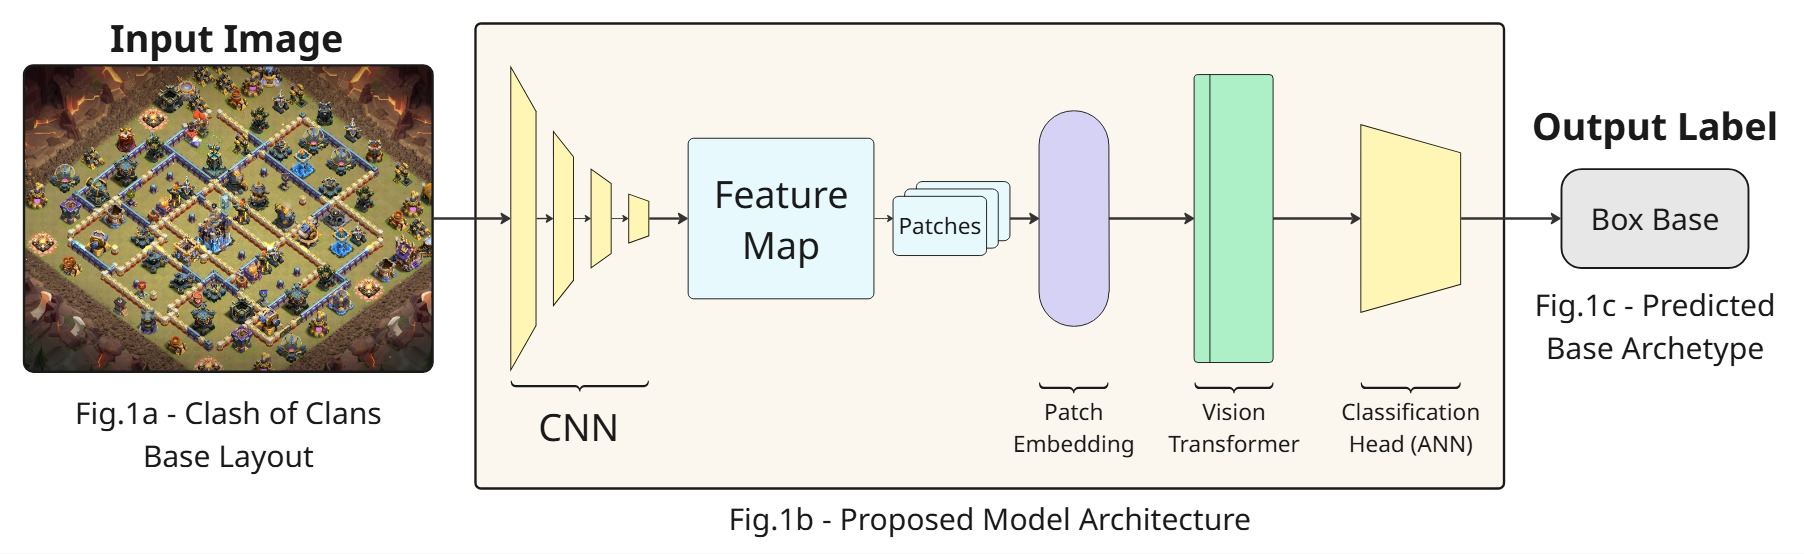
\includegraphics[width=1\textwidth]{diagram_proposed_arch.jpg}  % replace with your file name
  \caption{Proposed hybrid CNN-ViT model architecture.}
  \label{fig:architecture}
\end{figure}

% 4 marks
\section*{Background \& Related Work}

Listed below are some academic works that show why the proposed hybrid CNN-ViT model is suitable for this project:

1. \textbf{ImageNet Classification with Deep CNNs (AlexNet)} \cite{alexnet}: Showed that deep CNNs are effective in learning spatial features from images, making CNNs a strong backbone for the project.

2. \textbf{Deep Residual Learning (ResNet)} \cite{resnet}: Showed that ResNet can efficiently learn local features from residual connections. ResNet will be used as the CNN backbone for the model.

3. \textbf{Transformers for Image Recognition at Scale} \cite{tfir_vit1}: Showed that Vision Transformers (ViT) capture global image structure and are highly accurate for image classification.

4. \textbf{Introducing Convolutions into Vision Transformers} \cite{cvt}: Showed that combining ViTs with a CNN backbone increases performance and efficiency, making the architecture ideal for the project.

5. \textbf{Early Convolutions Help Transformers See Better} \cite{earlyconvvit}: Showed that a lightweight convolutional stem for the ViT models is a more robust architecture than standalone ViTs.

% 4 marks
\section*{Data Processing}

The dataset of base images will be collected from various sources. This includes CoC base sharing websites like Clash Champs \cite{clashchamps}, CoC Layouts \cite{coclayouts}, subreddits like r/COCBaseLayouts \cite{srcocbaselayouts}, and from personal base designs. Most of the data will be scraped and labeled per archetype using Python scripts, while some images from personal base designs and Reddit might require manual labeling. 

The resulting dataset will contain approximately 1000-2000 images. All images will be cropped and resized (e.g. 224x224 for ImageNet model compatibility) to ensure uniformity across samples. Images containing watermarks will be processed so that the watermark does not interfere with feature extraction. To increase the effective sample size and better model generalization, the cleaned dataset can be augmented through rotations (90\textdegree, 180\textdegree, 270\textdegree) expanding the dataset by up to four times.

% 2 marks
\section*{Architecture}

The proposed model uses a hybrid Convolutional Neural Network (CNN) and Vision Transformer (ViT) architecture. A pre-trained CNN (Eg. ResNet18/34 \cite{resnet}) will be used to extract local features from the input base images, such as wall patterns and compartments.

The resulting feature maps will be partitioned into patches and projected into embeddings through a patch embedding layer, allowing them to be processed by a ViT. The ViT captures global structural features of the base, which are necessary to identify the overall archetype. 

The output of the ViT is passed to a Feed-Forward neural net (classification head) which performs the base archetype classification. Depending on the dataset size and performance of the model, the later layers of the CNN may be fine-tuned as well. The overall architecture is depicted in Figure \ref{fig:architecture}b.


% 2 marks
\section*{Baseline Model}

The baseline model used for comparison will be a simple Artificial Neural Network (ANN). The input images will be flattened into a 1D tensor, passed through several layers with ReLU/Sigmoid activations, and finally passed through a softmax output layer for base archetype classification. The model will be trained using cross-entropy loss. The baseline model will be fast to train, but will lack the local feature capturing of the CNN and the global pattern recognition of the ViT.

Comparing the proposed model with the baseline would allow us to evaluate the benefits of the hybrid CNN-ViT model. The baseline ANN should converge quickly even on a smaller dataset, providing a good reference point for model performance.

% 2 marks
\section*{Ethical Considerations}

While the model is intended to assist players in planning and analyzing attack strategies, it should not be used to completely replace human decision making. In competitive Clash of Clans matches, especially in tournaments with cash prizes, use of such classification tools could give the user an unfair competitive advantage and may violate competition rules.

The dataset is collected from public base sharing websites which are biased towards popular competitive-style base designs. This could hinder the model's ability to classify novel and less common base archetypes. No personal information is collected from the data sources, only the base layouts and labels are collected. Therefore, the model poses minimal privacy risks.

\newpage
% \section*{References}
\bibliographystyle{unsrt}
\bibliography{references}

\end{document}